\documentclass[a4paper,14pt]{extarticle}

\usepackage[utf8x]{inputenc}
\usepackage[T1,T2A]{fontenc}
\usepackage[russian]{babel}
\usepackage{hyperref}
\usepackage{indentfirst}
\usepackage{here}
\usepackage{array}
\usepackage[table]{xcolor}
\usepackage{datetime}
\usepackage{multirow}
\usepackage{hhline}
\usepackage{mathtools,cancel}
\usepackage{forest}
\usepackage{graphicx}
\usepackage{caption}
\usepackage{subcaption}
\usepackage{chngcntr}
\usepackage{amsmath}
\usepackage{amssymb}
\usepackage{pgfplots}
\usepackage{pgfplotstable}
\usepackage[left=2cm,right=2cm,top=2cm,bottom=2cm,bindingoffset=0cm]{geometry}
\usepackage{multicol}
\usepackage{askmaps}
\usepackage{tikz}

\newcommand*\circled[1]{\tikz[baseline=(char.base)]{
            \node[shape=circle,draw,inner sep=2pt] (char) {#1};}}

\DeclareMathOperator*{\argmin}{argmin}

\renewcommand{\not}[1]{\mkern 1.5mu\overline{\mkern-1.5mu#1\mkern-1.5mu}\mkern 1.5mu}
\renewcommand{\le}{\ensuremath{\leqslant}}
\renewcommand{\leq}{\ensuremath{\leqslant}}
\renewcommand{\ge}{\ensuremath{\geqslant}}
\renewcommand{\geq}{\ensuremath{\geqslant}}
\renewcommand{\epsilon}{\ensuremath{\varepsilon}}
\renewcommand{\phi}{\ensuremath{\varphi}}

\counterwithin{figure}{section}
\counterwithin{equation}{section}
\counterwithin{table}{section}
\newcommand{\sign}[1][5cm]{\makebox[#1]{\hrulefill}} % Поля подписи и даты
\graphicspath{{pics/}} % Путь до папки с картинками
\captionsetup{justification=centering,margin=1cm}
\def\arraystretch{1.3}

\begin{document}

\begin{titlepage}
\begin{center}
	Санкт-Петербургский политехнический университет Петра Великого\\[0.3cm]
	Институт компьютерных наук и технологий \\[0.3cm]
	Кафедра компьютерных систем и программных технологий\\[4cm]
	
	\textbf{Расчётное задание №6}\\[2mm]
	\textbf{Дисциплина:} Системный анализ и принятие решений\\[2mm]
	\textbf{Тема:} Дискретное программирование. Задача коммивояжёра\\[2mm]
	Вариант 39\\[6.5cm]
\end{center}

\begin{flushleft}
	\hspace*{5mm} Выполнил студент гр. 33501/4  \hspace*{3cm}\sign[3cm]\hspace*{2mm} А.Ю. Ламтев\\
	\hspace*{10.85cm} (подпись)\\[2.5mm]
	\hspace*{5mm} Преподаватель \hspace*{6.45cm}\sign[3cm]\hspace*{2mm} С.С. Сабонис\\
	\hspace*{10.85cm} (подпись)\\[2.5mm]
	\hspace*{11.1cm} <<\underline{\the\day}>> \underline{\hspace{5mm}ноября\hspace{5mm}} \the\year\hspace{1mm} г.
\end{flushleft}

\vfill

\begin{center}
	Санкт-Петербург\\
	\the\year
\end{center}
\end{titlepage}
\addtocounter{page}{1}

\section{Задание}

Дана задача нелинейного программирования:

\begin{equation}
\label{eq:target}
	max \left( -17 x^2_1 - 23 x^2_2 + 8 x_1 x_2 + 182 x_1 + 266 x_2 \right)
\end{equation}

\begin{enumerate}

	\item Решить задачу методом Лагранжа при ограничении: 
	
		\begin{equation}
		\label{eq:lagrange-constraints}
			0 \cdot x_1 + 1 \cdot x_2 = 4
		\end{equation}
	
	\item Записать необходимые условия оптимальности для задачи при ограничениях:
	
		\begin{equation}
		\label{eq:bil-constraints}
			\begin{cases}
				9 x_1 + 7 x_2 \leq 63
				\\
				-x_1 + x_2 \leq 4
				\\
				-x_1 \leq 0
				\\
				-x_2 \leq 0
			\end{cases}
		\end{equation}
	
	\item Решить задачу методом Била при ограничениях \ref{eq:bil-constraints}.
	
	\item Решить задачу методом проекции градиента при ограничениях \ref{eq:bil-constraints}.	
	
	\item Записать необходимые условия оптимальности для задачи при ограничени:
	
	\begin{equation}
	\label{eq:quad-constraints}
		9 x_1^2 + 25 x_2^2 \leq 225
	\end{equation}

	\item Решить задачу методом штрафных функций при ограничении \ref{eq:quad-constraints}.
	
	\item Решить задачу методом возможных направлений Зойтендейка при ограничении \ref{eq:quad-constraints}.

\end{enumerate}

\section{Решение}

\subsection{Метод Лагранжа}

Запишем функцию Лагранжа для целевой функции \ref{eq:target} и заданного ограничения \ref{eq:lagrange-constraints}

\begin{equation*}
	L(X, V) = -17 x^2_1 - 23 x^2_2 + 8 x_1 x_2 + 182 x_1 + 266 x_2 + v(x_2 - 4)
\end{equation*}

Запишем условие стационарности $L(X, V)$ в точке $(X^*, V^*)$:

\begin{equation*}
	\begin{cases}
		\frac{\partial L}{\partial x_1} = -34 x_1 + 8 x_2 + 182 = 0
		\\
		\frac{\partial L}{\partial x_2} = -46 x_2 + 8 x_1 + 266 + v = 0
		\\
		\frac{\partial L}{\partial v} = x_2 - 4 = 0
	\end{cases}
\end{equation*}

Найдём $(X^*,\ V^*)$:

\begin{equation*}
	(X^*,\ V^*) = \left( \frac{107}{17},\ 4,\ -\frac{2250}{17} \right)
\end{equation*}

Вычислим матрицу Гессе для функции $L(X, V)$:

\begin{equation*}
	H = \begin{pmatrix}
		-34 & 8
		\\
		8 & -46
	\end{pmatrix}
\end{equation*}

Согласно критерию Сильвестра $H$ - отрицательно определённая. Следовательно $(X^*,\ V^*)$ -- точка максимума $L(X, V)$, а точка $X^* = \left(\frac{107}{17},\ 4 \right)$ -- решение поставленной задачи.

На рис. \ref{pic:lagrange} изображены линии уровня целевой функции и траектория поиска решения:

\begin{figure}[H]
\begin{center}
	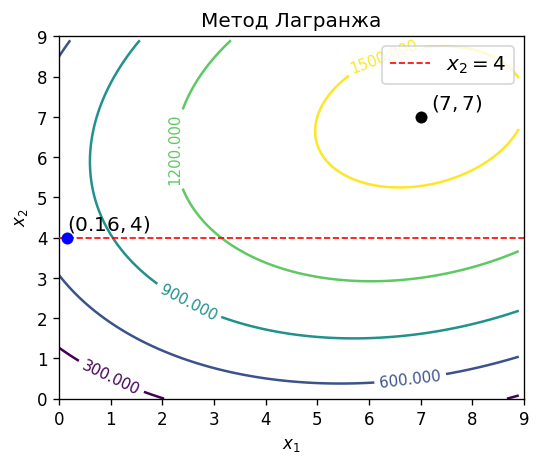
\includegraphics[scale=1]{lagrange}
	\caption{Линии равного уровня целевой функции и траектория поиска решения}
	\label{pic:lagrange}
\end{center}
\end{figure}

\subsection{Условия оптимальности для задачи с линейными ограничениями}

Запишем необходимые условия оптимальности для задачи с ограничениями \ref{eq:bil-constraints}. Преобразуем систему с ограничениями \ref{eq:bil-constraints} к следующему виду:

\begin{equation*}
	\begin{cases}
		9 x_1 + 7 x_2 - 63 \leq 0
		\\
		-x_1 + x_2 - 4 \leq 0
		\\
		x_1,\ x_2 \geq 0
	\end{cases}
\end{equation*}

В данном случае необходимым условием оптимальности будет следующее условие Куна-Такера:

\begin{equation}
\label{eq:kt}
	\begin{cases}
		f^{'}(X^*) + \sum\limits_{j = 1}^J u_j \cdot g^{'}_j(X^*) = 0
		\\
		u_j \cdot g_j(X^*) = 0,\ j = 1 \dots J
		\\
		u_j \leq 0,\ \text{если}\ g_j(X) \leq 0
		\\
		u_j \geq 0,\ \text{если}\ g_j(X) \geq 0
	\end{cases}
\end{equation}

Вычислим градиенты целевой функции и функций-ограничений:

\begin{equation*}
	\nabla f(X) = \left(  \frac{\partial f}{\partial x_1}(X) \hspace{7mm} \frac{\partial f}{\partial x_2}(X) \right)^T = \begin{pmatrix}
		-34 x_1 + 8 x_2 + 182
		\\
		-46 x_2 + 8 x_1 + 266
	\end{pmatrix}
\end{equation*}

\begin{equation*}
	\nabla g_1 = \left( 9 \hspace{5mm} 7 \right)^T
\end{equation*}

\begin{equation*}
	\nabla g_2 = \left( -1 \hspace{5mm} 1 \right)^T
\end{equation*}

\begin{equation*}
	\nabla g_3 = \left( 1 \hspace{5mm} 0 \right)^T
\end{equation*}

\begin{equation*}
	\nabla g_4 = \left( 0 \hspace{5mm} 1 \right)^T
\end{equation*}

Подставим вычисленные градиенты в уравнение \ref{eq:kt} и получим необходимые условия оптимальности $X^*$:

\begin{equation*}
	\begin{cases}
		\left( -34 x_1 + 8 x_2 + 182 \right) \Big|_{(x_1, x_2) = X^*} + u_1 \cdot 9 + u_2 \cdot (-1) + u_3 \cdot 1 + u_4 \cdot 0 = 0
		\\
		\left( -46 x_2 + 8 x_1 + 266 \right) \Big|_{(x_1, x_2) = X^*} + u_1 \cdot 7 + u_2 \cdot 1 + u_3 \cdot 0 + u_4 \cdot 1 = 0
		\\
		u_1 \cdot (9 x_1 + 7 x_2 - 63) \Big|_{(x_1, x_2) = X^*} = 0
		\\
		u_2 \cdot (-x_1 + x_2 - 4) \Big|_{(x_1, x_2) = X^*} = 0
		\\
		u_3 \cdot x_1 \Big|_{(x_1, x_2) = X^*} = 0
		\\
		u_4 \cdot x_2 \Big|_{(x_1, x_2) = X^*} = 0
		\\
		u_i \leq 0,\ i = 1,2
		\\
		u_j \geq 0,\ j = 3,4
	\end{cases}
\end{equation*}

\subsection{Метод Била}

Введём дополнительные переменные $x_3$ и $x_4$ и преобразуем систему ограничений \ref{eq:bil-constraints} к следующему виду:

\begin{equation*}
\begin{cases}
	9 x_1 + 7 x_2 + x_3 = 63
	\\
	- x_1 + x_2 + x_4 = 4
	\\
	x_i \geq 0,\ i = 1 \dots 4
\end{cases}
\end{equation*}

\paragraph{Шаг 1. Формирование начального базиса $\text{Б}_0$}

Пусть $\text{Б}_0 = (3,\ 4)$, тогда $X^{(0)} = (0,\ 0,\ 63,\ 4)^T$ -- допустимое базисное решение.

\paragraph{Шаг 2. Построение и анализ симплекс-таблицы.}

Построим симплекс-таблицу \ref{tab:simpl:1}:

\begin{table}[H]
\begin{center}
	\caption{Симплекс-таблица для базисного решения $X^{(0)}$}
	\label{tab:simpl:1}
	\def\tabcolsep{18pt}
	\def\arraystretch{1.5}
	\fontsize{13}{14}\selectfont
	\begin{tabular}{|c|c||c||c|}
		\hline 
		$X^{(0)}$ & $x_1$ & $x_2$ & $b$ \\ 
		\hline 
		$x_3$ & -9 & -7 & 63 \\ 
		\hhline{|=|=#=#=|}
		$x_4$ & 1 & \cellcolor{pink} -1 & 4 \\ 
		\hhline{|=|=#=#=|}
		$\frac{\partial f}{\partial x_r} \left(X^{(0)} \right)$ & 182 & 266 &  \\ 
		\hline 
	\end{tabular} 
\end{center}
\end{table}

Т.к. $c = (182\ \ 266)^T > 0$, базисное решение $X^{(0)}$ -- неоптимально.

Разрезающий столбец --- $x_2$, т.к. ей соответствует максимальная производная целевой функции --- 266.

Определим разрезающую строку. Для этого найдём соотношение между приращением свободной переменной $x_2$ и изменениями базисных переменных $x_3$, $x_4$ и производной $\frac{\partial f}{\partial x_2} \left(X \right)$:

\begin{equation*}
	\frac{\partial f}{\partial x_2} \left(X \right) = 0 \Rightarrow x_2 = \frac{266}{46} \approx 5.78
\end{equation*}

\begin{equation*}
	x_3 = 0\ \ \Rightarrow x_2 = \frac{63}{7} = 9
\end{equation*}

\begin{equation*}
	x_4 = 0\ \ \Rightarrow x_2 = \frac{4}{1} = 4
\end{equation*}

Переменная $x_4$ обращается в нуль раньше остальных, поэтому ей соответствует разрезающая строка.

Разрезающий элемент $-1$ выделен цветом в симплекс-таблице \ref{tab:simpl:1}. 

\paragraph{Шаг 3. Пересчёт симплекс-таблицы для базисного решения $X^{(1)}$.}

Пересчитаем симплекс-таблицу \ref{tab:simpl:1} и получим симплекс-таблицу \ref{tab:simpl:2}.

\begin{table}[H]
\begin{center}
	\caption{Симплекс-таблица для базисного решения $X^{(1)}$}
	\label{tab:simpl:2}
	\def\tabcolsep{18pt}
	\def\arraystretch{1.5}
	\fontsize{13}{14}\selectfont
	\begin{tabular}{|c||c||c|c|}
		\hline 
		$X^{(1)}$ & $x_1$ & $x_4$ & $b$ \\ 
		\hhline{|=#=#=|=|} 
		$x_3$ & \cellcolor{pink} -16 & 7 & 35 \\ 
		\hhline{|=#=#=|=|}
		$x_2$ & 1 & -1 & 4 \\ 
		\hline
		$\frac{\partial f}{\partial x_r} \left(X^{(1)} \right)$ & 296 & -82 &  \\ 
		\hline 
	\end{tabular} 
\end{center}
\end{table}

\begin{equation*}
\begin{aligned}
	f(X) = -17 x_1^2 - 23 (x_1 - x_4 + 4)^2 + 8 x_1 (x_1 - x_4 + 4) + 182 x_1 + 266 (x_1 - x_4 + 4) = \\ = -32 x_1^2 - 23 x_4^2 + 38 x_1 x_4 +296 x_1 - 82 x_4 + 696
\end{aligned}
\end{equation*}

\begin{equation*}
	\frac{\partial f}{\partial x_1} = -64 x_1 + 38 x_4 + 296
\end{equation*}

\begin{equation*}
	\frac{\partial f}{\partial x_4} = 38 x_1 -46 x_4 -82
\end{equation*}

Решение $X^{(1)} = (0,\ 4,\, 35,\ 0)^T$ --- допустимое, но не оптимальное, т.к. $c = (296\ \ -82)^T \nleq 0$.

Разрезающий столбец --- $x_1$, т.к. $x_1$ соответствует максимальная производная целевой функции --- 296.

Определим разрезающую строку. Для этого найдём соотношение между приращением свободной переменной $x_1$ и изменениями базисных переменных $x_2$, $x_3$ и производной $\frac{\partial f}{\partial x_1} \left(X \right)$:

\begin{equation*}
	\frac{\partial f(X)}{\partial x_1} = 0 \Rightarrow x_1 = \frac{296}{64} = 4.625
\end{equation*}

\begin{equation*}
	x_3 = 0\ \ \Rightarrow x_1 = \frac{35}{16} = 2.1875
\end{equation*}

\begin{equation*}
	x_2 = 0 \Rightarrow \ \ \ x_1 = -\frac{4}{1} = -4
\end{equation*}

Переменная $x_3$ обращается в нуль раньше остальных, поэтому ей соответствует разрезающая строка.

Разрезающий элемент $-16$ выделен цветом в симплекс-таблице \ref{tab:simpl:2}. 

\paragraph{Шаг 4. Пересчёт симплекс-таблицы для базисного решения $X^{(2)}$}

Пересчитаем симплекс-таблицу \ref{tab:simpl:2} и получим симплекс-таблицу \ref{tab:simpl:3}.

\begin{table}[H]
\begin{center}
	\caption{Симплекс-таблица для базисного решения $X^{(2)}$}
	\label{tab:simpl:3}
	\def\tabcolsep{18pt}
	\def\arraystretch{1.5}
	\fontsize{13}{14}\selectfont
	\begin{tabular}{|c|c||c||c|}
		\hline 
		$X^{(2)}$ & $x_3$ & $x_4$ & $b$ \\ 
		\hline
		$x_1$ & $-\frac{1}{16}$ & $\frac{7}{16}$ & $\frac{35}{16}$ \\ 
		\hline
		$x_2$ & $-\frac{1}{16}$ & -$\frac{9}{16}$ & $\frac{99}{16}$ \\ 
		\hline
		$\frac{\partial f}{\partial x_r} \left(X^{(2)} \right)$ & $-\frac{78}{8}$ & $\frac{555}{8}$ &  \\ 
		\hline 
	\end{tabular} 
\end{center}
\end{table}

\begin{equation*}
	f = \frac{1}{8} \left( -x_3^2 - 100 x_4^2 - 5 x_3 x_4 - 78 x_3 + 555 x_4 + 9523 \right)
\end{equation*}

\begin{equation*}
	\frac{\partial f}{\partial x_3} = \frac{1}{8} \left( -2 x_3 - 5 x_4 - 78 \right)
\end{equation*}

\begin{equation*}
	\frac{\partial f}{\partial x_4} = \frac{1}{8} \left( -5 x_3 - 200 x_4 + 555 \right)
\end{equation*}

Решение $X^{(2)} = \left(\frac{35}{16},\ \frac{99}{16} ,\, 0,\ 0\right)^T$ --- допустимое, но не оптимальное, т.к. $c = (-\frac{78}{8}\ \ \frac{555}{8})^T \nleq 0$.

Разрезающий столбец --- $x_4$, т.к. $x_4$ соответствует максимальная производная целевой функции --- $\frac{555}{8}$.

Определим разрезающую строку. Для этого найдём соотношение между приращением свободной переменной $x_4$ и изменениями базисных переменных $x_1$, $x_2$ и производной $\frac{\partial f}{\partial x_4} \left(X \right)$:

\begin{equation*}
	x_1 = 0\ \ \Rightarrow x_4 = -\frac{35}{16} \Big/ \frac{7}{16} = -5
\end{equation*}

\begin{equation*}
	x_2 = 0 \Rightarrow  x_4 = \frac{99}{16} \Big/ \frac{9}{16}= 11
\end{equation*}

\begin{equation*}
	\frac{\partial f(X)}{\partial x_4} = 0 \Rightarrow x_4 = \frac{555}{200} = 2.775
\end{equation*}

Производная$\frac{\partial f}{\partial x_4} \left(X \right)$ обращается в нуль раньше остальных, поэтому введём новую переменную $u_1$:

\begin{equation*}
	u_1 = \frac{1}{2} \frac{\partial f}{\partial x_4} = \frac{1}{16} \left( -5 x_3 - 200 x_4 + 555 \right)
\end{equation*}

Внесём её в симплекс-таблицу \ref{tab:simpl:4}:

\begin{table}[H]
\begin{center}
	\caption{Симплекс-таблица с $u_1$ для базисного решения $X^{(2)}$}
	\label{tab:simpl:4}
	\def\tabcolsep{18pt}
	\def\arraystretch{1.5}
	\fontsize{13}{14}\selectfont
	\begin{tabular}{|c|c||c||c|}
		\hline 
		$X^{(2)}$ & $x_3$ & $x_4$ & $b$ \\ 
		\hline
		$x_1$ & $-\frac{1}{16}$ & $\frac{7}{16}$ & $\frac{35}{16}$ \\ 
		\hline
		$x_2$ & $-\frac{1}{16}$ & -$\frac{9}{16}$ & $\frac{99}{16}$ \\ 
		\hhline{|=|=#=#=|}
		$u_1$ & $ -\frac{5}{16}$ & \cellcolor{pink} $-\frac{200}{16}$ & $\frac{555}{16}$ \\ 
		\hhline{|=|=#=#=|}
	\end{tabular} 
\end{center}
\end{table}

Разрезающий элемент $-\frac{200}{16}$ выделен цветом в симплекс-таблице \ref{tab:simpl:4}. 

\paragraph{Шаг 5. Пересчёт симплекс-таблицы для базисного решения $X^{(3)}$.}

Пересчитаем симплекс-таблицу \ref{tab:simpl:4} и получим симплекс-таблицу \ref{tab:simpl:5}.

\begin{table}[H]
\begin{center}
	\caption{Симплекс-таблица для базисного решения $X^{(3)}$}
	\label{tab:simpl:5}
	\def\tabcolsep{18pt}
	\def\arraystretch{1.5}
	\fontsize{13}{14}\selectfont
	\begin{tabular}{|c|c|c|c|}
		\hline 
		$X^{(3)}$ & $x_3$ & $u_1$ & $b$ \\ 
		\hline
		$x_1$ & $-\frac{235}{3200}$ & $-\frac{7}{3200}$ & \cellcolor{green} $\frac{10885}{3200} = 3.402$ \\ 
		\hline
		$x_2$ & $-\frac{155}{3200}$ & $\frac{9}{3200}$ & \cellcolor{green} $\frac{14805}{3200} = 4.627$ \\ 
		\hline
		$x_4$ & $ -\frac{5}{3200}$ & $-\frac{16}{200}$ & $\frac{555}{3200} = 0.173$ \\ 
		\hline
	\end{tabular} 
\end{center}
\end{table}

Решение $X^{(3)} = (3.402,\ 4.627,\, 0.173,\ 0)^T$ --- допустимое и оптимальное, т.к. $\frac{\partial f}{\partial x_3} (X^{(3)}) < 0$ и  $\frac{\partial f}{\partial u_1} (X^{(3)}) = 0$.

Решение исходной задачи:

\begin{equation*}
	X^{*} = \begin{pmatrix}
		3.402 \\ 4.627
	\end{pmatrix}
\end{equation*}

В таблице \ref{tab:bil} приведена траектория поиска решения:

\begin{table}[H]
\begin{center}
	\caption{Траектория поиска решения методом Била}
	\label{tab:bil}
	\def\tabcolsep{18pt}
	\def\arraystretch{1.5}
	\fontsize{13}{14}\selectfont
	\pgfplotstabletypeset[col sep=comma,
	    columns={i, x1, x2, f},
	    column type/.add={|c|}{},
	    columns/i/.style={fixed, precision=0, zerofill, column name={Шаг}},
	    columns/x1/.style={fixed, precision=3, zerofill, column name={$x_1$}},
	    columns/x2/.style={fixed, precision=3, zerofill, column name={$x_2$}},
	    columns/f/.style={fixed, precision=3, zerofill, column name={$f(X)$}},
	    every nth row={1}{before row=\hline},
	    every head row/.style={before row=\hline, after row=\hline, },
	    every last row/.style={after row=\hline}
	   ]{data/bil.csv}
\end{center}
\end{table}

На рис. \ref{pic:bil} изображены линии уровня целевой функции и траектория поиска решения:

\begin{figure}[H]
\begin{center}
	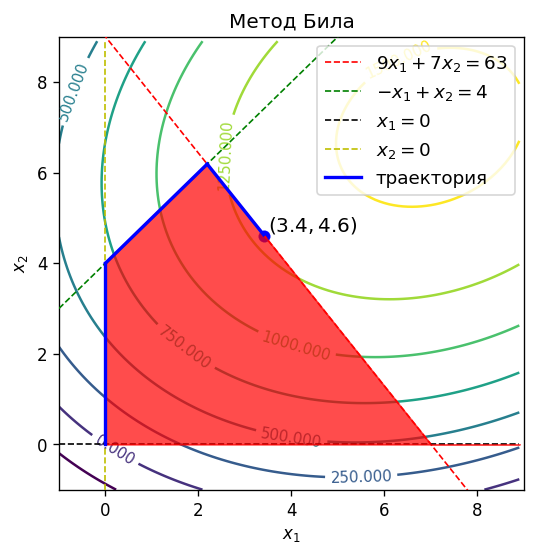
\includegraphics[scale=1]{bil}
	\caption{Линии равного уровня целевой функции и траектория поиска решения}
	\label{pic:bil}
\end{center}
\end{figure}

\subsection{Метод проекции градиента}

Запишем ограничения \ref{eq:bil-constraints} в матричной форме:

\begin{equation*}
	A \cdot X \leq b, 
\end{equation*}

\begin{equation*}
	A = \begin{pmatrix}
		9 & 7
		\\
		-1 & 1
		\\
		-1 & 0
		\\
		0 & -1
	\end{pmatrix}
	,\ %
	X = \begin{pmatrix}
	x_1 \\ x_2
	\end{pmatrix}
	,\ %
	b = \begin{pmatrix}
		63 \\ 4 \\ 0 \\ 0
	\end{pmatrix}
\end{equation*}

Вычислим градиент и гессиан целевой функции:

\begin{equation*}
	\nabla f(X) = \begin{pmatrix}
		-34 x_1 + 8 x_2 + 182
		\\
		-46 x_2 + 8 x_1 + 266
	\end{pmatrix}%
	,\ \ %
	H = \begin{pmatrix}
		-34 & 8
		\\
		8 & -46	
	\end{pmatrix}
\end{equation*}

В качестве начальной точки выберем $X^{(0)} = (0,\ 0)^T$

\paragraph{Шаг 1. Определение матрицы активных ограничений в начальной точке.}

Убедимся в допустимости градиентного направления:

\begin{equation*}
	A \nabla f(X^{(0)}) = \begin{pmatrix}
	-1 && 0 \\ 0 && -1
	\end{pmatrix}
	\begin{pmatrix}
	182 \\ 266
	\end{pmatrix}
	=
	\begin{pmatrix}
	-182 \\ -266
	\end{pmatrix}
	< 0,
\end{equation*}

поэтому $K^{(0)} = \nabla f(X^{(0)}) = \begin{pmatrix}
	182 & 266
	\end{pmatrix}^T$

\paragraph{Шаг 2. Выбор длины шага $t^{(0)}$}

Найдём множество $I_{prev}$ индексов нарушаемых ограничений.

\begin{equation*}
	A K^{(0)} = \begin{pmatrix}
		9 & 7
		\\
		-1 & 1
		\\
		-1 & 0
		\\
		0 & -1
	\end{pmatrix}
	\begin{pmatrix}
		182 \\ 266
	\end{pmatrix}
	=
	\begin{pmatrix}
		3500 \\ 84 \\ -182 \\ -266
	\end{pmatrix}
	\Rightarrow I_{prev} = \{1,\ 2\}
\end{equation*}

Тогда $t^{(0)} = min\{t^*,\ t_{prev_1},\ t_{prev_2}\}$

\begin{equation*}
	t^* = -\frac{\nabla^T f(X^{(0)}) K^{(0)}}{(K^{(0)})^T H K^{(0)}} = -\frac{(182\ 266) \begin{pmatrix} 182 \\ 266 \end{pmatrix}}{(182\ 266) \begin{pmatrix} -34 & 8 \\ 8 & -46 \end{pmatrix} \begin{pmatrix} 182 \\ 266 \end{pmatrix}} = 0.0288
\end{equation*}

\begin{equation*}
	t_{prev_1} = \frac{b_1 - a_1 X^{(0)}}{a_1 K^{(0)}} = \frac{63 - (9\ 7) \cdot 0}{(9\ 7) \begin{pmatrix} 182 \\ 266 \end{pmatrix}} = \frac{63}{3500} = 0.018
\end{equation*}

\begin{equation*}
	t_{prev_2} = \frac{b_2 - a_2 X^{(0)}}{a_2 K^{(0)}} = \frac{4 - (-1\ 1) \cdot 0}{(-1\ 1) \begin{pmatrix} 182 \\ 266 \end{pmatrix}} = \frac{4}{84} = 0.0476
\end{equation*}

\begin{equation*}
	t^{(0)} = t_{prev_1} = 0.018
\end{equation*}

\begin{equation*}
	X^{(1)} = X^{(0)} + t^{(0)} K^{(0)} = \begin{pmatrix}
		0 \\ 0 
	\end{pmatrix}
	+
	0.018 \cdot \begin{pmatrix}
		182 \\ 266 
	\end{pmatrix}
	=
	\begin{pmatrix}
		3.276 \\ 4.788
	\end{pmatrix}
\end{equation*}

\paragraph{Шаг 3. Формирование матрицы активных ограничений}

Определим оператор проекции и направлние $K^{(1)}$:

\begin{equation*}
	A = \begin{pmatrix} 9 & 7 \end{pmatrix},\ %
	\nabla f(X^{(1)}) = \begin{pmatrix} 108.92 & 71.96 \end{pmatrix}^T
\end{equation*}

\begin{equation*}
	A \nabla f(X^{(0)}) = \begin{pmatrix} 9 & 7 \end{pmatrix}
	\begin{pmatrix} 108.92 \\ 71.96 \end{pmatrix}
	=
	1484
	> 0,
\end{equation*}

направление градиента недопустимо.

\begin{equation*}
P = E - A^T \left(A A^T\right)^{-1} A = \begin{pmatrix} 1 & 0 \\ 0 & 1 \end{pmatrix} - \begin{pmatrix} 0.6231 & 0.4846 \\ 0.4846 & 0.3769 \end{pmatrix} = \begin{pmatrix} 0.3769 & -0.4846 \\ -0.4846 & 0.6231 \end{pmatrix}
\end{equation*}

\begin{equation*}
	K^{(1)} = P \nabla f(X^{(1)}) = \begin{pmatrix} 0.3769 & -0.4846 \\ -0.4846 & 0.6231 \end{pmatrix} \begin{pmatrix} 108.92 \\ 71.96 \end{pmatrix} = \begin{pmatrix} 6.18 \\ -7.94 \end{pmatrix}
\end{equation*}

\paragraph{Шаг 4. Выбор длины шага $t^{(1)}$}

Найдём множество $I_{prev}$ индексов нарушаемых ограничений.

\begin{equation*}
	A K^{(1)} = \begin{pmatrix}
		9 & 7
		\\
		-1 & 1
		\\
		-1 & 0
		\\
		0 & -1
	\end{pmatrix}
	\begin{pmatrix} 6.18 \\ -7.94 \end{pmatrix}
	=
	\begin{pmatrix}
		0.04 \\ -14.12 \\ -6.18 \\ 7.94
	\end{pmatrix}
	\Rightarrow I_{prev} = \{1,\ 4\}
\end{equation*}

Тогда $t^{(1)} = min\{t^*,\ t_{prev_4}\}$

\begin{equation*}
	t^* = -\frac{\nabla^T f(X^{(1)}) K^{(1)}}{(K^{(1)})^T H K^{(1)}} = -\frac{(108.92\  71.96) \begin{pmatrix} 6.18 \\ -7.94 \end{pmatrix}}{(6.18\ -7.94) \begin{pmatrix} -34 & 8 \\ 8 & -46 \end{pmatrix} \begin{pmatrix} 6.18 \\ -7.94 \end{pmatrix}} = 0.0204
\end{equation*}

%\begin{equation*}
%	t_{prev_1} = \frac{b_1 - a_1 X^{(1)}}{a_1 K^{(1)}} = \frac{63 - (9\ 7) \cdot \begin{pmatrix} 3.276 \\ 4.788 \end{pmatrix}}{(9\ 7) \begin{pmatrix} 6.18 \\ -7.94 \end{pmatrix}} = \frac{4.8678}{9.369} = 0.519
%\end{equation*}

\begin{equation*}
	t_{prev_4} = \frac{b_4 - a_4 X^{(1)}}{a_4 K^{(1)}} = \frac{0 - (0\ -1) \cdot \begin{pmatrix} 3.276 \\ 4.788 \end{pmatrix}}{(0\ -1) \begin{pmatrix} 6.18 \\ -7.94 \end{pmatrix}} = \frac{4.788}{7.94} = 0.6
\end{equation*}

\begin{equation*}
	t^{(1)} = t^* = 0.0204
\end{equation*}

\begin{equation*}
	X^{(2)} = X^{(1)} + t^{(1)} K^{(1)} = \begin{pmatrix}
		3.276 \\ 4.788
	\end{pmatrix}
	+
	0.0204 \cdot \begin{pmatrix} 6.18 \\ -7.94 \end{pmatrix}
	=
	\begin{pmatrix}
		3.4 \\ 4.6
	\end{pmatrix}
\end{equation*}

\paragraph{Шаг 5. Выбор направления}

\begin{equation*} 
	\nabla f(X^{(2)}) = \begin{pmatrix} 
		103.44
		\\ 
		80.22
	\end{pmatrix}
\end{equation*}

\begin{equation*}
	K^{(2)} = P \nabla f(X^{(2)}) = \begin{pmatrix} 
		0.3769 & -0.4846 
		\\ 
		-0.4846  & 0.6231 
	\end{pmatrix}
	\begin{pmatrix} 
		103.44
		\\ 
		80.22
	\end{pmatrix}
	=
	\begin{pmatrix} 
		0.111924 \\-0.141942
	\end{pmatrix}
\end{equation*}

\paragraph{Шаг 6. Выбор длины шага $t^{(2)}$}

\begin{equation*}
	A K^{(2)} = \begin{pmatrix}
		9 & 7
		\\
		-1 & 1
		\\
		-1 & 0
		\\
		0 & -1
	\end{pmatrix}
	\begin{pmatrix} 
		-0.0172
		\\ 
		0.0241
	\end{pmatrix}
	=
	\begin{pmatrix}
		0.014 \\ 0.041 \\ 0.017\\ -0.024
	\end{pmatrix}
	\Rightarrow I_{prev} = \{1,\ 2,\ 3\}
\end{equation*}

Тогда $t^{(2)} = min\{t^*,\ t_{prev_1}\}$

\begin{equation*}
	t^* = -\frac{\nabla^T f(X^{(2)}) K^{(2)}}{(K^{(2)})^T H K^{(2)}} = -\frac{(101.13\  78.69) \begin{pmatrix} -0.0172 \\ 0.0241 \end{pmatrix}}{(-0.0172\ 0.0241) \begin{pmatrix} -34 & 8 \\ 8 & -46 \end{pmatrix} \begin{pmatrix} -0.0172 \\ 0.0241 \end{pmatrix}} = 396
\end{equation*}

\begin{equation*}
	t_{prev_1} = \frac{b_1 - a_1 X^{(2)}}{a_1 K^{(2)}} = \frac{63 - (0\ -1) \cdot \begin{pmatrix} 3.3306 \\ 4.8678 \end{pmatrix}}{(0\ -1) \begin{pmatrix} 7.288 \\ -9.369 \end{pmatrix}} = \frac{4.8678}{9.369} = 0.519
\end{equation*}

\begin{equation*}
	t^{(2)} = t^* = 0.02033
\end{equation*}

\begin{equation*}
	X^{(2)} = X^{(1)} + t^{(1)} K^{(1)} = \begin{pmatrix}
		3.3306 \\ 4.8678
	\end{pmatrix}
	+
	0.02033 \cdot \begin{pmatrix} 7.288 \\ -9.369 \end{pmatrix}
	=
	\begin{pmatrix}
		3.402 \\ 4.627
	\end{pmatrix}
\end{equation*}

\paragraph{Шаг 7. Проверка условий останова}

Найдём вектор $\Lambda = - \left( A A^T \right)^{-1} A \nabla f (X^{(2)})$

\begin{equation*}
\begin{aligned}
	\Lambda = -\left( \begin{pmatrix} 9 && 7 \end{pmatrix} \begin{pmatrix} 9 \\ 7 \end{pmatrix} \right)^{-1} \begin{pmatrix} 9 && 7 \end{pmatrix} \begin{pmatrix} 107.13 \\ 78.69 \end{pmatrix} = - 11.65 < 0 \Rightarrow \\ \Rightarrow X^{(2)} = \begin{pmatrix}
		3.402 \\ 4.627
	\end{pmatrix}\ \text{-- оптимальное решение}
\end{aligned}
\end{equation*}

\begin{equation*}
	X^{*} = \begin{pmatrix}
		3.402 \\ 4.627
	\end{pmatrix}
\end{equation*}

В таблице \ref{tab:projection} приведена траектория поиска решения:

\begin{table}[H]
\begin{center}
	\caption{Траектория поиска решения методом проекции градиента}
	\label{tab:projection}
	\def\tabcolsep{18pt}
	\def\arraystretch{1.5}
	\fontsize{13}{14}\selectfont
	\pgfplotstabletypeset[col sep=comma,
	    columns={i, x1, x2, f},
	    column type/.add={|c|}{},
	    columns/i/.style={fixed, precision=0, zerofill, column name={Шаг}},
	    columns/x1/.style={fixed, precision=3, zerofill, column name={$x_1$}},
	    columns/x2/.style={fixed, precision=3, zerofill, column name={$x_2$}},
	    columns/f/.style={fixed, precision=3, zerofill, column name={$f(X)$}},
	    every nth row={1}{before row=\hline},
	    every head row/.style={before row=\hline, after row=\hline, },
	    every last row/.style={after row=\hline}
	   ]{data/projection.csv}
\end{center}
\end{table}

На рис. \ref{pic:projection} изображены линии уровня целевой функции и траектория поиска решения:

\begin{figure}[H]
\begin{center}
	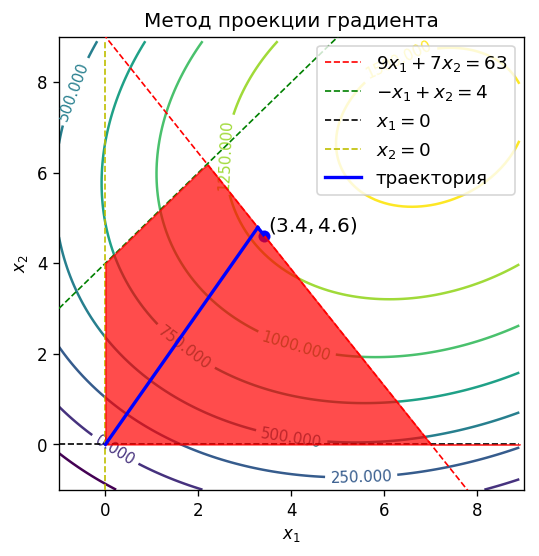
\includegraphics[scale=1]{projection}
	\caption{Линии равного уровня целевой функции и траектория поиска решения}
	\label{pic:projection}
\end{center}
\end{figure}

\subsection{Условия оптимальности для задачи с нелинейными ограничениями}

Запишем необходимые условия оптимальности для задачи с ограничениями \ref{eq:quad-constraints}. В данном случае необходимым условием оптимальности будет следующее условие Куна-Такера:

\begin{equation*}
\begin{cases}
	\frac{\partial f}{\partial x_1} + u_1 \frac{\partial g_1}{\partial x_1} = 0
	\\
	\frac{\partial f}{\partial x_2} + u_1 \frac{\partial g_1}{\partial x_2} = 0
	\\
	u_1 g_1 = 0
	\\
	u_1 \leq 0
\end{cases}
\end{equation*}

Подставим в него данные из ограничений \ref{eq:quad-constraints}:

\begin{equation*}
\begin{cases}
	-34 x_1 + 8 x_2 + 188 + 18 x_1 u_1 = 0
	\\
	-46 x_2 + 8 x_1 + 266 + 50 x_2 u_1 = 0
	\\
	u_1 g_1 = 0
	\\
	u_1 \leq 0
\end{cases}
\end{equation*}

\subsection{Метод штрафных функций}

Решим задачу методом штрафных функций при ограничении \ref{eq:quad-constraints}. Для этого обозначим ограничение функцией:

\begin{equation*}
	g(X) = 9 x_1^2 + 25 x_2^2 - 225
\end{equation*}

Вместо задачи условной оптимизации будем решать эквивалентную задачу безусловной оптимизации. Введём штрафную функцию $F(x)$ и штраф за нарушение ограничений исходной задачи $\psi(x)$:

\begin{equation*}
\psi(x) = \max \left\{ 0, x \right\}
\end{equation*}
\begin{equation*}
F(X, \mu) = f(X) - \mu \psi(g(X))
\end{equation*}

В таблице \ref{tab:penalty} приведена траектория поиска решения методом штрафных функций.

\begin{table}[H]
\begin{center}
	\caption{Траектория поиска решения методом штрафных функций}
	\label{tab:penalty}
	\def\tabcolsep{18pt}
	\def\arraystretch{1.5}
	\fontsize{13}{14}\selectfont
	\pgfplotstabletypeset[col sep=comma,
	    columns={i,mu, x1, x2, f},
	    column type/.add={|c|}{},
	    columns/i/.style={string type, column name={Шаг}},
	    columns/mu/.style={fixed, precision=3, zerofill, column name={$\mu$}},
	    columns/x1/.style={fixed, precision=3, zerofill, column name={$x_1$}},
	    columns/x2/.style={fixed, precision=3, zerofill, column name={$x_2$}},
	    columns/f/.style={fixed, precision=3, zerofill, column name={$f(X)$}},
	    every nth row={1}{before row=\hline},
	    every head row/.style={before row=\hline, after row=\hline, },
	    every last row/.style={after row=\hline}
	   ]{data/penalty.csv}
\end{center}
\end{table}

На рис. \ref{pic:penalty} изображены линии уровня целевой функции и траектория поиска решения:

\begin{figure}[H]
\begin{center}
	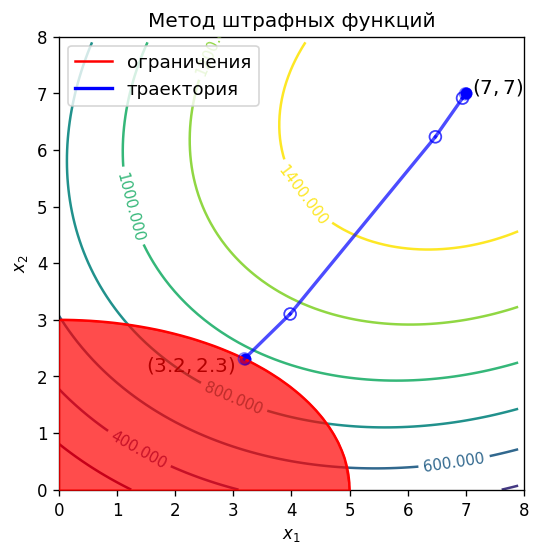
\includegraphics[scale=1]{penalty}
	\caption{Линии равного уровня целевой функции и траектория поиска решения}
	\label{pic:penalty}
\end{center}
\end{figure}

\subsection{Метод возможных направлений Зойтендейка}

Решим задачу методом возможных направлений Зойтендейка при ограничении \ref{eq:quad-constraints}.

При поиске на границе области формулируется вспомогательная задача линейного программирования:
\begin{equation*}
\begin{cases}
	\max(u)
	\\
	\left\langle f'(X^{(i)}, K^{(i)} \right\rangle \geq u
	\\
	\left\langle g_l'(X^{(i)}, K^{(i)} \right\rangle \geq u, l \in I
	\\
	u \geq 0,\ -1 \leq K_J^{(i)} \leq 1,\ j = 1 \dots n
\end{cases}
\end{equation*}

В таблице \ref{tab:penalty} приведена траектория поиска решения методом возможных направлений.

\begin{table}[H]
\begin{center}
	\caption{Траектория поиска решения методом возможных направлений}
	\label{tab:available}
	\def\tabcolsep{18pt}
	\def\arraystretch{1.0}
	\fontsize{13}{14}\selectfont
	\pgfplotstabletypeset[col sep=comma,
	    columns={i, x1, x2, u, f, k1, k2},
	    column type/.add={|c|}{},
	    columns/i/.style={string type, column name={Шаг}},
	    columns/x1/.style={fixed, precision=3, zerofill, column name={$x_1$}},
	    columns/x2/.style={fixed, precision=3, zerofill, column name={$x_2$}},
	    columns/u/.style={fixed, precision=3, zerofill, column name={$u$}},
	    columns/f/.style={fixed, precision=3, zerofill, column name={$f(X)$}},
	    columns/k1/.style={fixed, precision=3, zerofill, column name={$k_1$}},
	    columns/k2/.style={fixed, precision=3, zerofill, column name={$k_2$}},
	    every nth row={1}{before row=\hline},
	    every head row/.style={before row=\hline, after row=\hline, },
	    every last row/.style={after row=\hline}
	   ]{data/available.csv}
\end{center}
\end{table}

На рис. \ref{pic:available} --- \ref{pic:available-zoom} изображены линии уровня целевой функции и траектория поиска решения крупным планом и в приближении соответственно:

\begin{figure}[H]
\begin{center}
	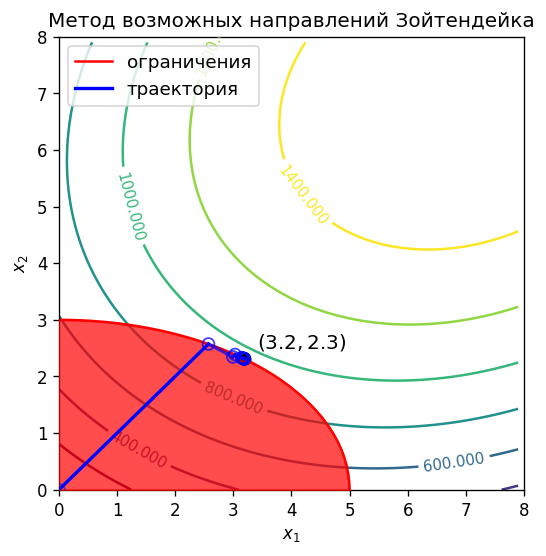
\includegraphics[scale=0.91]{available}
	\caption{Линии равного уровня целевой функции и траектория поиска решения}
	\label{pic:available}
\end{center}
\end{figure}

\begin{figure}[H]
\begin{center}
	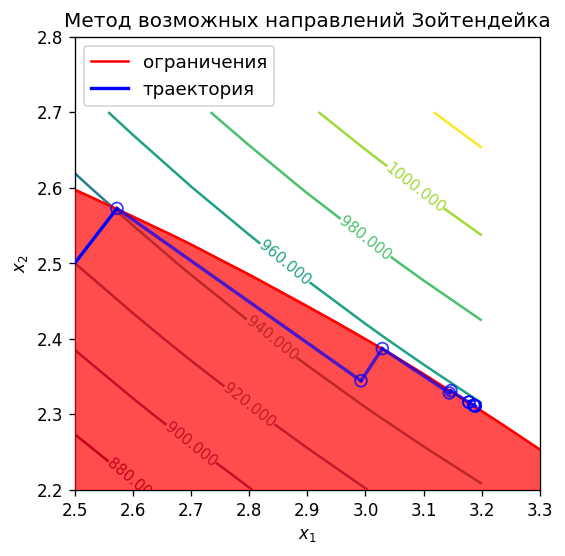
\includegraphics[scale=1]{available_zoom}
	\caption{Линии равного уровня целевой функции и траектория поиска решения}
	\label{pic:available-zoom}
\end{center}
\end{figure}

\end{document}